\documentclass[11pt,a4paper]{report}
\usepackage[utf8]{inputenc}
\usepackage{amsmath}
\usepackage{amsfonts}
\usepackage{amssymb}
\usepackage{graphicx}
\usepackage[nottoc]{tocbibind}
\usepackage[semicolon]{natbib}
\usepackage{url}
\usepackage{listings}
\def\UrlBreaks{\do\/\do-}
\usepackage{breakurl}
\usepackage[breaklinks]{hyperref}
\bibliographystyle{unsrtnat}
\author{Aedan Lawrence \\\ \href{mailto:Aedan.Lawrence.2019@live.rhul.ac.uk}{Aedan.Lawrence.2019@live.rhul.ac.uk}}
\title{Combating Fake News Using Mobile Trusted Execution Environments}
\date{EPMS School, Royal Holloway University of London, Egham TW20 0PW, UK}
\begin{document}
\maketitle
\tableofcontents
\newpage
\section{Abstract}
\textbf{On messaging apps such as WhatsApp, news can get shared into large groups, which people can and do take a face value without critically thinking.} If a malicious figure were to pretend to be a trusted news agency, this could spread fake news very quickly. Therefore, we need a way to detect fake news trying to masquerade as a trusted news source.

Fake news has gained a large amount of publicity over the recent years; however, current detection methods use language analysis and some common sense. Language analysis can be a minimal way to try and detect fake news meaning people still have to try and make an educated guess as to whether that news source is authentic.

An approach to fixing this is to design and prototype a system that allows a server to receive a link, check that link compared to a list of the news source, verify that the news source indeed wrote that article and therefore sign the article using a private key which would allow the messaging group to know that this comes from an authentic news source taking out some of the guessing work in spotting fake news. This checking could also be offloaded to the phone’s TEE chip, making it even more secure.

Finally, this solution on its own is a tiny step in stopping the spread of fake news and is not a one-stop solution. However, mixed with other pre-existing technologies to detect fake news, it is a stepping stone in limiting its effects.
\newpage
\section{Introduction}
Fake news has been an issue for many years, it is getting increasingly prevalent in everyday life, and therefore detection methods need to get better and more accurate. A report by First Draft News \citep{Fakenews} identified seven distinct types of fake news these are:
\begin{enumerate}
  \item satire or parody.
  \item false connection.
  \item misleading content.
  \item false context.
  \item imposter content.
  \item manipulated content.
  \item fabricated content.
\end{enumerate}
Typically, most news will come from social media and messaging applications, and this can give people in charge of groups on these sites a large amount of power over what news people see, share, and read. As of 2021, 13\% of all consumed news is from Facebook alone (Team, 2021). With the rise in influence social media has over our lives, whether political, such as the 2016 US election or medical-related such as during the COVID-19 pandemic, we need to manage and correctly identify information from these sites. Facebook started this during the pandemic, flagging miss-leading news as potentially inaccurate on all social media platforms it owned.

The plan is to help identify news sources that are satire or parody in nature and impostor content, as both are detectable based upon the URL and certificates. A system like this would be implementable into most social media and messaging apps and flag articles as potentially imposter or known satire content. Something like this is beneficial as want to be imposters can easily make their domain look something like bbc.a.co.uk, which may be hard to spot anything that would suggest that is not the BBC for the typical person.

The project started by planning a system to implement which looks something like this:
\begin{center}
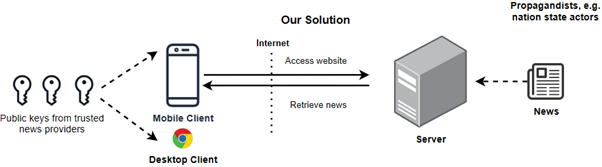
\includegraphics[width=1\textwidth]{image/diagram.png}
\end{center}
The plan here is that when a URL is shared of an expected news website, the phone will send a request to the server.

As I will only be prototyping this system due to time constants, I picked Flask for python as the framework for the server. Flask allows for rapid changes and easy development. As well as Flask, I will be using the cryptography module for python as this allows the server to sign the news content using ECDSA (Elliptic Curve Digital Signature Algorithm). Finally, I also plan to use SQLAlchemy to store the keys that each publisher can use.

Why ECDSA? ECDSA, while being less commonly used overall, is more complicated due to its asymmetry, which means it is harder to revert. “ECDSA provides the same level of security as RSA, but it does so while using much shorter key lengths. Therefore, for longer keys, ECDSA takes considerably more time to crack through brute-forcing attacks.” \citep{RSA}. It can, however, be harder overall to implement, which may cause issues in development.

Once this is working, the next task will be to modify an Android application to use the signing server when it detects a news article shared on the platform. An easy proof of concept way to do this will be to detect and check all URL’s that are shared on the platform. This way, all news content will be flagged, and non-news links will be marked with a warning.

Once a URL is detected, a query to the signing server needs to be made, providing the URL is shared via social media. The URL detection allows the signing server to try and match that URL with known good news sources; if it can find that article on a news site, we know that it is a genuine article and not an imposter article. 

Once found, the signing server will sign the URL and return that information to the requesting application. It is then up to the application to check the signature using the server’s public key and, at that point, can confirm to the user that this is indeed news from the claimed publisher.

Parody news sites are checkable in the same way, but the returning information will have an additional flag to mark it as parody content. Parody checking then allows the end-user application to flag it as a known parody site.

Using the phone’s built-in TEE (Trusted Execution Environment) chip to decode the signature, we can add another layer of security, making this system much harder to penetrate. A TEE system could be modelled on Linux using OP-TEE (Open Portable Trusted Execution Environment).

According to OP-TEE’s documentation, “it helps to separate the non-secure OS and user apps from the secure code which is baked into the hardware” \citep{OP-TEE}. TEE would allow the singing verification code to run securely without the worry of being tampered with and, therefore, will help to have an even higher level of validity for the news checking.

Once finished with the working prototype of the signing server and Android application, the next task will be to look at prototyping an OP-TEE application that decodes the signature so that in a perfect world, the three would become an active verification service with the security of TEE (Trusted Execution Environment).
\newpage
\section{Development and Difficulties}
\subsection{Flask Server}
The python server implementation was smooth and required little coding expertise in this proof of concept method.

A critical issue that showed its head early on was the lack of free and publicly accessible APIs (Application Programming Interfaces) from publishers; this limited the project’s number of working sites in the prototype. Due to not having the time to email each publisher separately, I used two API’s I could get by just signing up publicly. These were the New York Times and The Guardian. I would have had access to all news publishers in a perfect world instead of just these two.

The lack of API’s was also an issue for spotting a satirical/parody news website as it meant I could only spot them using string matching on the domain name and therefore could not check whether it was just a parody news site or an imposter site pretending to be a parody news website. However, this is not the end of the world as it still detects most parody websites, and worst case, they will be flagged as possibly imposter/uncheckable instead of a parody.

In the end, I fixed both issues by writing an API for all news websites. By storing the certificates of a trusted news source, I can compare the incoming URL with my certificate store, and if there is a match and the URL returns a 200-response code, the server can sign the news with confidence. The API allows me to check websites that do not provide an API.

Now I can add public keys of trusted news sources to my database, and I can start verifying all news sources.

A working JSON reply can look like this:
\begin{center}
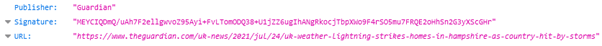
\includegraphics[width=1\textwidth]{image/json1.png}
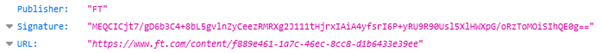
\includegraphics[width=1\textwidth]{image/json2.png}
\end{center}
Another issue I faced was sharing the public key so that the mobile client could easily access it. Flask only allows returns to be a string, dict, tuple, Response instance or WSGI callable, which meant I struggled to share the key. I found I could share the public key in bytes form using the public\_bytes() method built into the EC (Elliptic Curve) Cryptography package with a bit of research. Typically, this would not be an issue as the public key would be collected from a trusted certificate store and therefore would not need to be shared by the server.

However, after playing with this for a while, I realised I was wasting my time and should have been hard coding the public key to verify the signature as it does not need to change or expire for testing purposes; therefore, the key is within the Java application.
\subsection{Signal Application}
The next challenge was to pick an application to modify to implement this system. The obvious choice would have been Messenger and WhatsApp. Both were closed source, which led me to find that Signal \citep{Signal} has outstanding open-source support. As it is effectively a mirror application of WhatsApp, however not belonging to Facebook, it was a suitable candidate to show an example implementation.

First, I had to isolate the URL handling part of Signal, filtering through methods in Android Studio, which led me to find linkpreview in the securesms package. The methods in the LinkPreviewUtil class are called every time a preview for a URL needs to be loaded. By modifying this class, I can get access to just the URL part of the message sent.

Next, while in a development stage, I disabled the requirement for the HTTPS certificate to be stored with a certificate store as this is a requirement for Android apps; however would have just cost me money to test this idea, having not done much android app development before I also disabled the requirement for URL responses to be made using background threads as it was simpler just to wait for a response. Once I had a working verification method, I put the requests to my server in an AsyncTask, which allowed me to reenable Android’s thread requirements.

AsyncTask allows me to send the needed requests to the server when Signal detects a link, and this allows the requests to run in the background without limiting the application. The next step is to take the provided information from the server and, using java’s built-in security packages, recreate the public key and verify the provided signature.

While reconstructing the public key and signature in java, I had a tough time getting a working, parseable public key. After doing some research, this is due to how hazmat cryptography handles EC encryption by default vs how Java Security handles EC encryption.

While Python has excellent support for different types of curves, java on Android does not. Due to these differences, I was providing java with a secp256k1 curve from which java could create a public key; however, it could not use the public key to verify the signature. One of the few curve’s java supports is secp256r1, so once I converted my server key to this format, java could easily verify the signature. \citep{Exception}.

Finally, this meant I could verify news sources sent via Signal on Android. If an URL is pretending to be a news source that it is not, then it will not be verified. At this moment in time, it only is verifiable using the ADB logs and does not have a visual display element. To get a visual display, I need to add a Snackbar to the application; this will allow for a small pop up to alert the user if the news source is valid or not.
\newpage
\subsection{Current Known Bugs and Limitations}
\begin{enumerate}
  \item Not all news websites can be added to my API, as the way I read the public certificate does not work with all certificates for some reason.
  \item The URL is checked every time the preview for a URL is loaded, and this means if the news site goes down after it has been sent and received once, it could later be flagged as possible imposter news.
  \item The NYTimes is using their API, which limits me to being able to check the top 20 articles of the day. On the other hand, The Guardian’s API seems to fail for some articles for no apparent reason.
  \item All network request that goes through signal will accept their certificates even if they are self-signed currently due to the implementation of talking to my server. This is not secure!
  \item Due to time constraints, all code is not heavily debugged and can error on edge cases when it should not.
\end{enumerate}
\newpage
\section{Conclusion and Reflection}
\textbf{Overall, I think this project has gone quite well in its current state as the fundamental problem of manually spot impostor news has been accomplished.} Also, adding the ability to spot satire news helps to stop the spread of miss information, even if unintentionally.

However, as of the time writing this report, I have not yet had the opportunity to look at or start to implement OP-TEE. Due to this there is still a bit of work to make the system more secure. If I were to start this project again, I would work on this implementation before the Android one as the two are linked. This could be started by running OP-TEE on QEMU to emulate an arm device.

Another implementation of this system would be to get it added to bigger/other social media applications and desktop add on for web browsers. This would allow news links on any website to be checked for imposter/satire content; while not helpful for all users, this may be helpful for older generations as a web browser.

I also spent too long research and not asking enough questions, which wasted my own time as I would be trying to implement ideas that were not needed and not helpful. As this was such a practical based UROP (Undergraduate Research Opportunities), if I were to do it again, I would jump straight into development and research at the same time instead of a few weeks of research followed by a few weeks of coding. I would also have a higher interaction with my lectures which would help to mitigate these issues.

Nevertheless, another thing that could be done would be to combine this detection system with a language analysis method of detecting fake news, as this would allow many more websites to be flagged for things that are not just imposter content.

I am, however, happy with the technologies I had learned and used to use along the way, such as elliptical curve encryption, Flask servers and android app development, as these are all things which before the project, I had either not done or done to a much lower level.
\newpage
\section{Code availability}
The python server code can be found here: \\ \url{https://github.com/MrInterBugs/Combatting-Fake-News} \\ To run this code use: \\ \textbf{flask run --cert=cert.pem --key=key.pem --host=0.0.0.0} \\ \\ The modified signal code can be found here: \\ \url{https://github.com/MrInterBugs/Signal-Android}
\newpage
\bibliography{References}
\end{document}